\documentclass[14pt]{extbook}
\usepackage{multicol, enumerate, enumitem, hyperref, color, soul, setspace, parskip, fancyhdr} %General Packages
\usepackage{amssymb, amsthm, amsmath, latexsym, units, mathtools} %Math Packages
\everymath{\displaystyle} %All math in Display Style
% Packages with additional options
\usepackage[headsep=0.5cm,headheight=12pt, left=1 in,right= 1 in,top= 1 in,bottom= 1 in]{geometry}
\usepackage[usenames,dvipsnames]{xcolor}
\usepackage{dashrule}  % Package to use the command below to create lines between items
\newcommand{\litem}[1]{\item#1\hspace*{-1cm}\rule{\textwidth}{0.4pt}}
\pagestyle{fancy}
\lhead{Makeup Progress Quiz 2}
\chead{}
\rhead{Version ALL}
\lfoot{2790-1423}
\cfoot{}
\rfoot{Summer C 2021}
\begin{document}

\begin{enumerate}
\litem{
Solve the linear equation below. Then, choose the interval that contains the solution.\[ \frac{3x + 7}{8} - \frac{-7x + 7}{5} = \frac{4x -7}{2} \]\begin{enumerate}[label=\Alph*.]
\item \( x \in [21.67, 26.67] \)
\item \( x \in [13.22, 15.22] \)
\item \( x \in [28.11, 33.11] \)
\item \( x \in [-2.5, 0.5] \)
\item \( \text{There are no real solutions.} \)

\end{enumerate} }
\litem{
Find the equation of the line described below. Write the linear equation in the form $ y=mx+b $ and choose the intervals that contain $m$ and $b$.\[ \text{Perpendicular to } 4 x - 7 y = 9 \text{ and passing through the point } (10, -5). \]\begin{enumerate}[label=\Alph*.]
\item \( m \in [-2.94, -1.6] \hspace*{3mm} b \in [11.5, 16.5] \)
\item \( m \in [-2.94, -1.6] \hspace*{3mm} b \in [-14.5, -9.5] \)
\item \( m \in [-2.94, -1.6] \hspace*{3mm} b \in [-18, -14] \)
\item \( m \in [-1.18, 0.03] \hspace*{3mm} b \in [11.5, 16.5] \)
\item \( m \in [1.29, 2.87] \hspace*{3mm} b \in [-23.5, -16.5] \)

\end{enumerate} }
\litem{
Write the equation of the line in the graph below in Standard Form $Ax+By=C$. Then, choose the intervals that contain $A, B, \text{ and } C$.
\begin{center}
    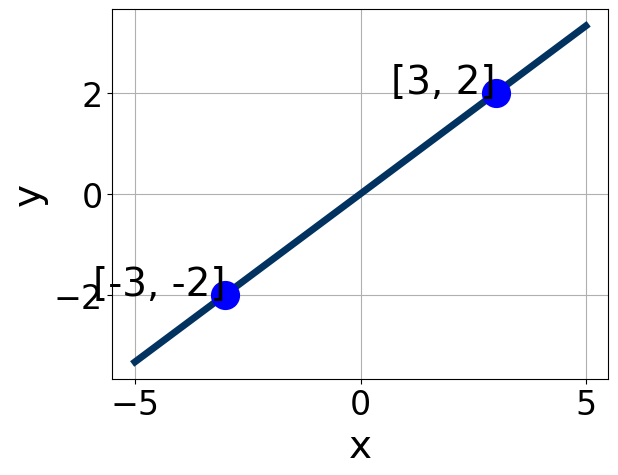
\includegraphics[width=0.5\textwidth]{../Figures/linearGraphToStandardCopyA.png}
\end{center}
\begin{enumerate}[label=\Alph*.]
\item \( A \in [1.4, 2.2], \hspace{3mm} B \in [2.31, 3.13], \text{ and } \hspace{3mm} C \in [0, 1] \)
\item \( A \in [-1.1, 1.8], \hspace{3mm} B \in [-2.36, -0.31], \text{ and } \hspace{3mm} C \in [0, 1] \)
\item \( A \in [1.4, 2.2], \hspace{3mm} B \in [-4.83, -2.98], \text{ and } \hspace{3mm} C \in [0, 1] \)
\item \( A \in [-1.1, 1.8], \hspace{3mm} B \in [0.09, 1.2], \text{ and } \hspace{3mm} C \in [0, 1] \)
\item \( A \in [-2.1, -1.8], \hspace{3mm} B \in [2.31, 3.13], \text{ and } \hspace{3mm} C \in [0, 1] \)

\end{enumerate} }
\litem{
First, find the equation of the line containing the two points below. Then, write the equation in the form $ y=mx+b $ and choose the intervals that contain $m$ and $b$.\[ (-6, 6) \text{ and } (-11, -10) \]\begin{enumerate}[label=\Alph*.]
\item \( m \in [0.2, 4.2] \hspace*{3mm} b \in [-27.2, -20.2] \)
\item \( m \in [0.2, 4.2] \hspace*{3mm} b \in [6, 16] \)
\item \( m \in [0.2, 4.2] \hspace*{3mm} b \in [1, 2] \)
\item \( m \in [0.2, 4.2] \hspace*{3mm} b \in [24.2, 27.2] \)
\item \( m \in [-3.2, -2.2] \hspace*{3mm} b \in [-48.2, -42.2] \)

\end{enumerate} }
\litem{
Solve the equation below. Then, choose the interval that contains the solution.\[ -17(-16x -18) = -7(-5x -9) \]\begin{enumerate}[label=\Alph*.]
\item \( x \in [-1.71, -1.38] \)
\item \( x \in [-1.38, -1.03] \)
\item \( x \in [-1.04, -0.79] \)
\item \( x \in [1.39, 1.7] \)
\item \( \text{There are no real solutions.} \)

\end{enumerate} }
\litem{
First, find the equation of the line containing the two points below. Then, write the equation in the form $ y=mx+b $ and choose the intervals that contain $m$ and $b$.\[ (9, -6) \text{ and } (-2, -2) \]\begin{enumerate}[label=\Alph*.]
\item \( m \in [-1.08, -0.24] \hspace*{3mm} b \in [-0.3, 0.13] \)
\item \( m \in [-1.08, -0.24] \hspace*{3mm} b \in [2.21, 3.36] \)
\item \( m \in [-0.18, 1.45] \hspace*{3mm} b \in [-1.84, -0.28] \)
\item \( m \in [-1.08, -0.24] \hspace*{3mm} b \in [-15.44, -14.63] \)
\item \( m \in [-1.08, -0.24] \hspace*{3mm} b \in [-2.91, -2.1] \)

\end{enumerate} }
\litem{
Solve the linear equation below. Then, choose the interval that contains the solution.\[ \frac{-3x + 8}{2} - \frac{-3x -3}{4} = \frac{-8x -4}{7} \]\begin{enumerate}[label=\Alph*.]
\item \( x \in [-9.73, -7.73] \)
\item \( x \in [-1.67, 1.33] \)
\item \( x \in [-39.18, -34.18] \)
\item \( x \in [-13.55, -10.55] \)
\item \( \text{There are no real solutions.} \)

\end{enumerate} }
\litem{
Find the equation of the line described below. Write the linear equation in the form $ y=mx+b $ and choose the intervals that contain $m$ and $b$.\[ \text{Perpendicular to } 5 x + 9 y = 9 \text{ and passing through the point } (2, 9). \]\begin{enumerate}[label=\Alph*.]
\item \( m \in [1.63, 2.26] \hspace*{3mm} b \in [-6.8, -4.4] \)
\item \( m \in [0.53, 0.7] \hspace*{3mm} b \in [2.5, 6.9] \)
\item \( m \in [1.63, 2.26] \hspace*{3mm} b \in [6.8, 7.5] \)
\item \( m \in [1.63, 2.26] \hspace*{3mm} b \in [2.5, 6.9] \)
\item \( m \in [-2.2, -1.18] \hspace*{3mm} b \in [11.5, 12.7] \)

\end{enumerate} }
\litem{
Write the equation of the line in the graph below in Standard Form $Ax+By=C$. Then, choose the intervals that contain $A, B, \text{ and } C$.
\begin{center}
    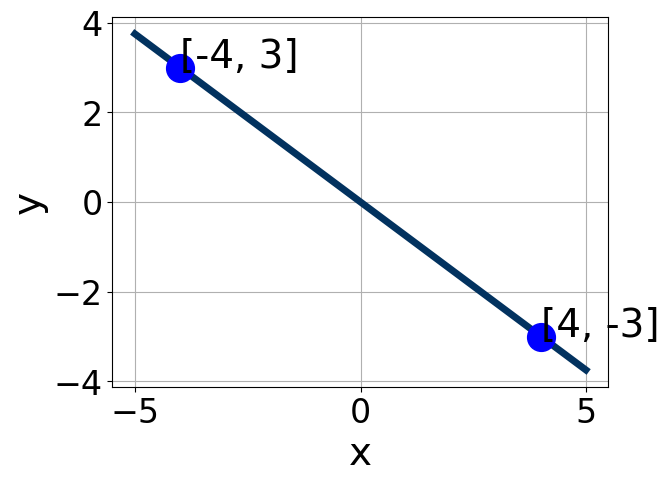
\includegraphics[width=0.5\textwidth]{../Figures/linearGraphToStandardA.png}
\end{center}
\begin{enumerate}[label=\Alph*.]
\item \( A \in [2.2, 4.6], \hspace{3mm} B \in [-5.6, -2.4], \text{ and } \hspace{3mm} C \in [0, 4] \)
\item \( A \in [0.3, 1], \hspace{3mm} B \in [-0.8, 1.4], \text{ and } \hspace{3mm} C \in [0, 4] \)
\item \( A \in [-5.2, -2.4], \hspace{3mm} B \in [-5.6, -2.4], \text{ and } \hspace{3mm} C \in [0, 4] \)
\item \( A \in [2.2, 4.6], \hspace{3mm} B \in [3.7, 4.6], \text{ and } \hspace{3mm} C \in [0, 4] \)
\item \( A \in [0.3, 1], \hspace{3mm} B \in [-2, -0.5], \text{ and } \hspace{3mm} C \in [0, 4] \)

\end{enumerate} }
\litem{
Solve the equation below. Then, choose the interval that contains the solution.\[ -10(-8x -4) = -15(6x -12) \]\begin{enumerate}[label=\Alph*.]
\item \( x \in [-1.68, -0.73] \)
\item \( x \in [0.72, 1.17] \)
\item \( x \in [1.2, 1.78] \)
\item \( x \in [21.99, 22.46] \)
\item \( \text{There are no real solutions.} \)

\end{enumerate} }
\litem{
Solve the linear equation below. Then, choose the interval that contains the solution.\[ \frac{5x + 3}{4} - \frac{7x + 5}{8} = \frac{5x + 4}{6} \]\begin{enumerate}[label=\Alph*.]
\item \( x \in [-13.2, -11.3] \)
\item \( x \in [1.2, 1.8] \)
\item \( x \in [-1.7, -0.9] \)
\item \( x \in [-1, 0.6] \)
\item \( \text{There are no real solutions.} \)

\end{enumerate} }
\litem{
Find the equation of the line described below. Write the linear equation in the form $ y=mx+b $ and choose the intervals that contain $m$ and $b$.\[ \text{Perpendicular to } 3 x + 4 y = 4 \text{ and passing through the point } (-7, 3). \]\begin{enumerate}[label=\Alph*.]
\item \( m \in [0.97, 1.75] \hspace*{3mm} b \in [9, 12] \)
\item \( m \in [-1.67, -0.91] \hspace*{3mm} b \in [-7.33, -5.33] \)
\item \( m \in [0.97, 1.75] \hspace*{3mm} b \in [-19.33, -11.33] \)
\item \( m \in [0.66, 1.09] \hspace*{3mm} b \in [12.33, 15.33] \)
\item \( m \in [0.97, 1.75] \hspace*{3mm} b \in [12.33, 15.33] \)

\end{enumerate} }
\litem{
Write the equation of the line in the graph below in Standard Form $Ax+By=C$. Then, choose the intervals that contain $A, B, \text{ and } C$.
\begin{center}
    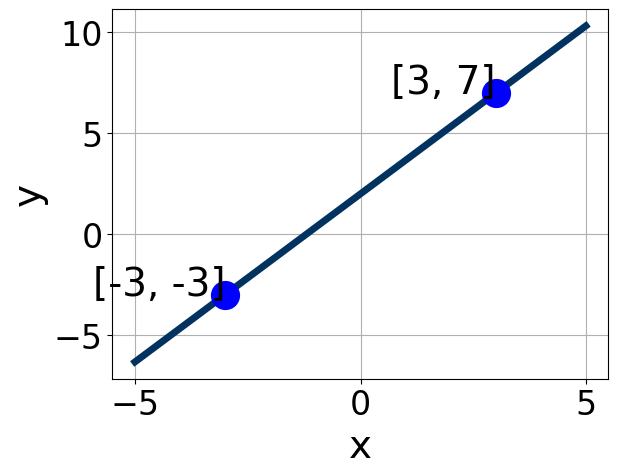
\includegraphics[width=0.5\textwidth]{../Figures/linearGraphToStandardCopyB.png}
\end{center}
\begin{enumerate}[label=\Alph*.]
\item \( A \in [3.8, 6.1], \hspace{3mm} B \in [1.6, 3.2], \text{ and } \hspace{3mm} C \in [5.2, 6.9] \)
\item \( A \in [-6, -4.7], \hspace{3mm} B \in [1.6, 3.2], \text{ and } \hspace{3mm} C \in [5.2, 6.9] \)
\item \( A \in [-2.8, -1.3], \hspace{3mm} B \in [-1.96, 0.04], \text{ and } \hspace{3mm} C \in [-5.7, -1] \)
\item \( A \in [-2.8, -1.3], \hspace{3mm} B \in [-0.43, 1.42], \text{ and } \hspace{3mm} C \in [1.2, 3.9] \)
\item \( A \in [3.8, 6.1], \hspace{3mm} B \in [-5.33, -1.85], \text{ and } \hspace{3mm} C \in [-7.2, -4.8] \)

\end{enumerate} }
\litem{
First, find the equation of the line containing the two points below. Then, write the equation in the form $ y=mx+b $ and choose the intervals that contain $m$ and $b$.\[ (-11, 8) \text{ and } (2, 2) \]\begin{enumerate}[label=\Alph*.]
\item \( m \in [-1.54, 0.12] \hspace*{3mm} b \in [-4.35, -2.3] \)
\item \( m \in [-1.54, 0.12] \hspace*{3mm} b \in [18.24, 19.45] \)
\item \( m \in [-1.54, 0.12] \hspace*{3mm} b \in [-0.88, 0.95] \)
\item \( m \in [-1.54, 0.12] \hspace*{3mm} b \in [2.36, 3.43] \)
\item \( m \in [-0.35, 1.07] \hspace*{3mm} b \in [1.04, 1.74] \)

\end{enumerate} }
\litem{
Solve the equation below. Then, choose the interval that contains the solution.\[ -3(12x + 17) = -4(18x -7) \]\begin{enumerate}[label=\Alph*.]
\item \( x \in [-0.46, 0.59] \)
\item \( x \in [-1.71, -0.3] \)
\item \( x \in [0.58, 1.15] \)
\item \( x \in [2.03, 2.62] \)
\item \( \text{There are no real solutions.} \)

\end{enumerate} }
\litem{
First, find the equation of the line containing the two points below. Then, write the equation in the form $ y=mx+b $ and choose the intervals that contain $m$ and $b$.\[ (11, 2) \text{ and } (5, -3) \]\begin{enumerate}[label=\Alph*.]
\item \( m \in [-0.2, 1.7] \hspace*{3mm} b \in [-8.08, -7.75] \)
\item \( m \in [-0.2, 1.7] \hspace*{3mm} b \in [6.77, 8.18] \)
\item \( m \in [-0.2, 1.7] \hspace*{3mm} b \in [-9.51, -8.91] \)
\item \( m \in [-0.2, 1.7] \hspace*{3mm} b \in [-7.19, -6.58] \)
\item \( m \in [-3.5, -0.4] \hspace*{3mm} b \in [0.75, 1.58] \)

\end{enumerate} }
\litem{
Solve the linear equation below. Then, choose the interval that contains the solution.\[ \frac{5x -3}{6} - \frac{7x + 4}{3} = \frac{-5x -5}{4} \]\begin{enumerate}[label=\Alph*.]
\item \( x \in [7.5, 9.7] \)
\item \( x \in [-1, 0.4] \)
\item \( x \in [-8.8, -6.4] \)
\item \( x \in [-2.5, -1.5] \)
\item \( \text{There are no real solutions.} \)

\end{enumerate} }
\litem{
Find the equation of the line described below. Write the linear equation in the form $ y=mx+b $ and choose the intervals that contain $m$ and $b$.\[ \text{Perpendicular to } 7 x + 3 y = 8 \text{ and passing through the point } (-8, 2). \]\begin{enumerate}[label=\Alph*.]
\item \( m \in [2.15, 2.99] \hspace*{3mm} b \in [4.8, 6.6] \)
\item \( m \in [0.34, 0.8] \hspace*{3mm} b \in [8.3, 12.4] \)
\item \( m \in [0.34, 0.8] \hspace*{3mm} b \in [-5.9, -3] \)
\item \( m \in [0.34, 0.8] \hspace*{3mm} b \in [4.8, 6.6] \)
\item \( m \in [-0.91, -0.08] \hspace*{3mm} b \in [-1.6, -0.9] \)

\end{enumerate} }
\litem{
Write the equation of the line in the graph below in Standard Form $Ax+By=C$. Then, choose the intervals that contain $A, B, \text{ and } C$.
\begin{center}
    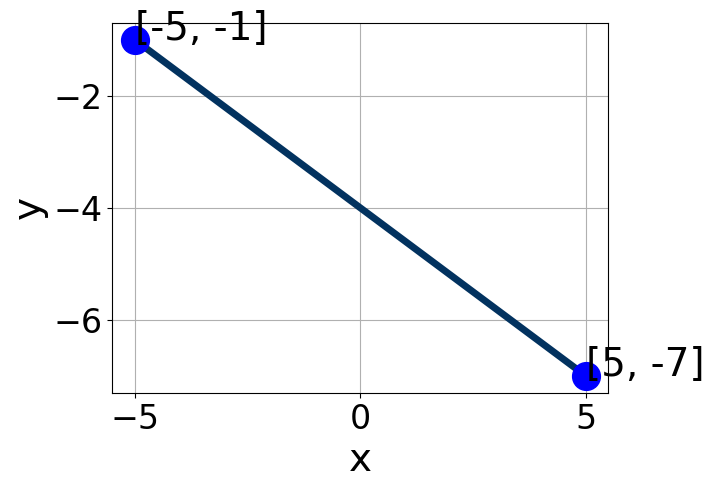
\includegraphics[width=0.5\textwidth]{../Figures/linearGraphToStandardB.png}
\end{center}
\begin{enumerate}[label=\Alph*.]
\item \( A \in [-0.2, 2.6], \hspace{3mm} B \in [0.71, 1.37], \text{ and } \hspace{3mm} C \in [-8, -1] \)
\item \( A \in [1.9, 5.1], \hspace{3mm} B \in [-5.68, -4.25], \text{ and } \hspace{3mm} C \in [20, 25] \)
\item \( A \in [-0.2, 2.6], \hspace{3mm} B \in [-1.54, 0.53], \text{ and } \hspace{3mm} C \in [4, 9] \)
\item \( A \in [-3.8, -2.3], \hspace{3mm} B \in [-5.68, -4.25], \text{ and } \hspace{3mm} C \in [20, 25] \)
\item \( A \in [1.9, 5.1], \hspace{3mm} B \in [4.46, 6.38], \text{ and } \hspace{3mm} C \in [-21, -17] \)

\end{enumerate} }
\litem{
Solve the equation below. Then, choose the interval that contains the solution.\[ -13(15x -11) = -4(-6x + 5) \]\begin{enumerate}[label=\Alph*.]
\item \( x \in [0.53, 0.57] \)
\item \( x \in [0.74, 0.76] \)
\item \( x \in [-0.59, -0.55] \)
\item \( x \in [0.71, 0.74] \)
\item \( \text{There are no real solutions.} \)

\end{enumerate} }
\litem{
Solve the linear equation below. Then, choose the interval that contains the solution.\[ \frac{4x + 3}{4} - \frac{4x -7}{3} = \frac{6x -7}{6} \]\begin{enumerate}[label=\Alph*.]
\item \( x \in [-0.78, -0.3] \)
\item \( x \in [3.1, 3.85] \)
\item \( x \in [12.36, 13.67] \)
\item \( x \in [0, 1.28] \)
\item \( \text{There are no real solutions.} \)

\end{enumerate} }
\litem{
Find the equation of the line described below. Write the linear equation in the form $ y=mx+b $ and choose the intervals that contain $m$ and $b$.\[ \text{Perpendicular to } 9 x + 7 y = 7 \text{ and passing through the point } (-8, -5). \]\begin{enumerate}[label=\Alph*.]
\item \( m \in [0.39, 1.13] \hspace*{3mm} b \in [-1.5, 0.4] \)
\item \( m \in [-1.48, -0.33] \hspace*{3mm} b \in [-14.6, -10.5] \)
\item \( m \in [0.39, 1.13] \hspace*{3mm} b \in [0.3, 2] \)
\item \( m \in [0.39, 1.13] \hspace*{3mm} b \in [2.4, 3.9] \)
\item \( m \in [0.87, 1.62] \hspace*{3mm} b \in [0.3, 2] \)

\end{enumerate} }
\litem{
Write the equation of the line in the graph below in Standard Form $Ax+By=C$. Then, choose the intervals that contain $A, B, \text{ and } C$.
\begin{center}
    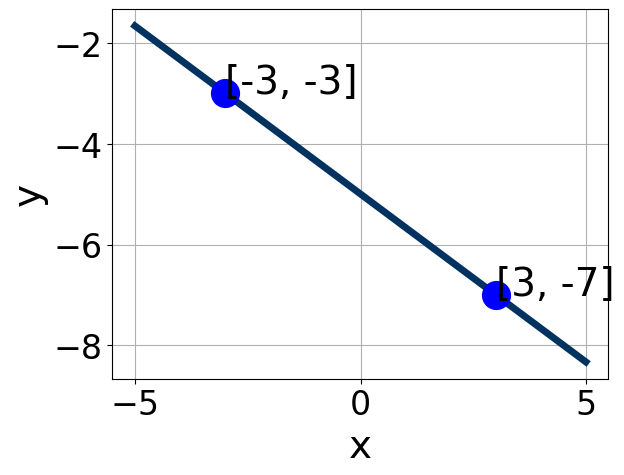
\includegraphics[width=0.5\textwidth]{../Figures/linearGraphToStandardCopyC.png}
\end{center}
\begin{enumerate}[label=\Alph*.]
\item \( A \in [0.4, 0.9], \hspace{3mm} B \in [-1.1, -0.84], \text{ and } \hspace{3mm} C \in [5, 6] \)
\item \( A \in [0.8, 2.4], \hspace{3mm} B \in [-3.16, -2.12], \text{ and } \hspace{3mm} C \in [9, 17] \)
\item \( A \in [0.8, 2.4], \hspace{3mm} B \in [1.85, 3.9], \text{ and } \hspace{3mm} C \in [-17, -8] \)
\item \( A \in [-2.2, -1.2], \hspace{3mm} B \in [-3.16, -2.12], \text{ and } \hspace{3mm} C \in [9, 17] \)
\item \( A \in [0.4, 0.9], \hspace{3mm} B \in [-0.47, 1.93], \text{ and } \hspace{3mm} C \in [-8, 1] \)

\end{enumerate} }
\litem{
First, find the equation of the line containing the two points below. Then, write the equation in the form $ y=mx+b $ and choose the intervals that contain $m$ and $b$.\[ (-2, -5) \text{ and } (6, 9) \]\begin{enumerate}[label=\Alph*.]
\item \( m \in [0.75, 3.75] \hspace*{3mm} b \in [-0.24, 1.69] \)
\item \( m \in [0.75, 3.75] \hspace*{3mm} b \in [-3.9, -2.15] \)
\item \( m \in [-7.75, -0.75] \hspace*{3mm} b \in [19.05, 20.67] \)
\item \( m \in [0.75, 3.75] \hspace*{3mm} b \in [2.13, 4.37] \)
\item \( m \in [0.75, 3.75] \hspace*{3mm} b \in [-1.63, -0.94] \)

\end{enumerate} }
\litem{
Solve the equation below. Then, choose the interval that contains the solution.\[ -2(-13x -11) = -14(-5x -18) \]\begin{enumerate}[label=\Alph*.]
\item \( x \in [-6, -4.9] \)
\item \( x \in [-4, -2.6] \)
\item \( x \in [-8, -6] \)
\item \( x \in [6, 6.9] \)
\item \( \text{There are no real solutions.} \)

\end{enumerate} }
\litem{
First, find the equation of the line containing the two points below. Then, write the equation in the form $ y=mx+b $ and choose the intervals that contain $m$ and $b$.\[ (7, -9) \text{ and } (-7, -11) \]\begin{enumerate}[label=\Alph*.]
\item \( m \in [-1.06, -0.12] \hspace*{3mm} b \in [-14, -10.2] \)
\item \( m \in [0.11, 0.46] \hspace*{3mm} b \in [8.9, 10.1] \)
\item \( m \in [0.11, 0.46] \hspace*{3mm} b \in [-10.3, -8.9] \)
\item \( m \in [0.11, 0.46] \hspace*{3mm} b \in [-16.5, -15.2] \)
\item \( m \in [0.11, 0.46] \hspace*{3mm} b \in [-6, -3.8] \)

\end{enumerate} }
\litem{
Solve the linear equation below. Then, choose the interval that contains the solution.\[ \frac{5x + 6}{7} - \frac{6x + 9}{4} = \frac{-9x + 9}{8} \]\begin{enumerate}[label=\Alph*.]
\item \( x \in [32.37, 36.37] \)
\item \( x \in [-0.69, 2.31] \)
\item \( x \in [-7.84, -4.84] \)
\item \( x \in [6.42, 9.42] \)
\item \( \text{There are no real solutions.} \)

\end{enumerate} }
\litem{
Find the equation of the line described below. Write the linear equation in the form $ y=mx+b $ and choose the intervals that contain $m$ and $b$.\[ \text{Parallel to } 3 x + 7 y = 10 \text{ and passing through the point } (-2, 4). \]\begin{enumerate}[label=\Alph*.]
\item \( m \in [-0.55, -0.28] \hspace*{3mm} b \in [5.6, 6.9] \)
\item \( m \in [0.05, 0.95] \hspace*{3mm} b \in [4, 5.3] \)
\item \( m \in [-0.55, -0.28] \hspace*{3mm} b \in [-3.3, -1.6] \)
\item \( m \in [-0.55, -0.28] \hspace*{3mm} b \in [1.3, 4.7] \)
\item \( m \in [-2.72, -2.15] \hspace*{3mm} b \in [1.3, 4.7] \)

\end{enumerate} }
\litem{
Write the equation of the line in the graph below in Standard Form $Ax+By=C$. Then, choose the intervals that contain $A, B, \text{ and } C$.
\begin{center}
    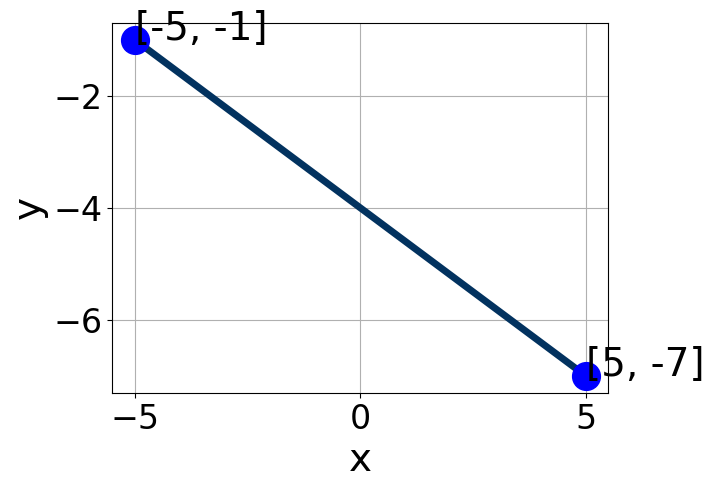
\includegraphics[width=0.5\textwidth]{../Figures/linearGraphToStandardC.png}
\end{center}
\begin{enumerate}[label=\Alph*.]
\item \( A \in [-3.54, -2.69], \hspace{3mm} B \in [-5.8, -2.9], \text{ and } \hspace{3mm} C \in [18, 23] \)
\item \( A \in [2.92, 3.89], \hspace{3mm} B \in [-5.8, -2.9], \text{ and } \hspace{3mm} C \in [18, 23] \)
\item \( A \in [0.48, 1.46], \hspace{3mm} B \in [-3.5, -0.2], \text{ and } \hspace{3mm} C \in [2, 5] \)
\item \( A \in [0.48, 1.46], \hspace{3mm} B \in [-0.1, 4.1], \text{ and } \hspace{3mm} C \in [-4, -2] \)
\item \( A \in [2.92, 3.89], \hspace{3mm} B \in [2.4, 6.8], \text{ and } \hspace{3mm} C \in [-20, -15] \)

\end{enumerate} }
\litem{
Solve the equation below. Then, choose the interval that contains the solution.\[ -19(6x -13) = -17(8x -18) \]\begin{enumerate}[label=\Alph*.]
\item \( x \in [25.07, 25.17] \)
\item \( x \in [-25.73, -24.72] \)
\item \( x \in [2.45, 2.86] \)
\item \( x \in [1.77, 2.63] \)
\item \( \text{There are no real solutions.} \)

\end{enumerate} }
\end{enumerate}

\end{document}